% !TeX program = pdflatex
% Complete article, End Matter, supporting derivations and bibliography in this file.
% Overleaf: select this file as Main document; compiler pdfLaTeX, TeX Live 2025.
% Rebuild the quantitative plot locally: python Graph/generate_plots.py
% Then compile twice: pdflatex -interaction=nonstopmode -halt-on-error Quantum_Precision_Heat_Tradeoff_arXiv.tex
% No shell escape, external TeX inputs, BibTeX, or network access is required.
% Scientific baseline: f749753c5000bfa3efb3466d67c12b4b1befbb4b.
% Repository: https://github.com/GoGoKo699/Quantum-Precision-Heat-Tradeoff
\documentclass[aps,prl,reprint,amsmath,amssymb,superscriptaddress,longbibliography]{revtex4-2}
\usepackage{amsmath,amssymb,bm,graphicx,booktabs}
\usepackage[T1]{fontenc}
\usepackage[utf8]{inputenc}
\usepackage{microtype}
\usepackage{hyperref}
\usepackage{orcidlink}
\hypersetup{colorlinks=true,linkcolor=blue,citecolor=blue,urlcolor=blue,
 pdftitle={Finite Heat at Vanishing Entropy Change in Quantum Operations},
 pdfauthor={Ranyiliu Chen; Ruge Lin},pdfsubject={Precision-dependent microscopic heat in quantum operations}}
\newcommand{\Tr}{\operatorname{Tr}}
\newcommand{\rank}{\operatorname{rank}}
\newcommand{\supp}{\operatorname{supp}}
\newcommand{\atanh}{\operatorname{atanh}}
\newcommand{\id}{\operatorname{id}}
\newcommand{\JS}{\operatorname{JS}}
\newcommand{\ket}[1]{\lvert #1\rangle}
\newcommand{\bra}[1]{\langle #1\rvert}
\newcommand{\proj}[1]{\ket{#1}\!\bra{#1}}
\newcommand{\norm}[1]{\lVert #1\rVert}
\newcommand{\dd}{\mathrm d}
\newcommand{\eps}{\epsilon}
\newcommand{\kb}{k_{\mathrm B}}
\newcommand{\Ucal}{\mathcal U}
\newcommand{\Ncal}{\mathcal N}
\newcommand{\Tcal}{\mathcal T}
\newcommand{\Dcal}{\mathcal D}
\newcommand{\Hcal}{\mathcal H}
\newcommand{\J}{J_2}
\newcommand{\Db}{D_2}
\newcommand{\qmin}{q_{\min}}
\newcommand{\qdiamond}{q_{\min}^{\diamond}}
\newcommand{\para}[1]{\textit{#1.}\quad}
\newcommand{\papertitle}{Finite Heat at Vanishing Entropy Change in Quantum Operations}
\setlength{\emergencystretch}{1.5em}
\allowdisplaybreaks[1]

% Author order and affiliations supplied by the authors.
\newcommand{\HKUSTGZ}{\affiliation{Thrust of Artificial Intelligence, Information Hub, The Hong Kong University of Science and Technology (Guangzhou), Guangzhou 511453, China}}
\newcommand{\QSC}{\affiliation{Quantum Science Center of Guangdong-Hong Kong-Macao Greater Bay Area, Shenzhen 518045, China}}

\usepackage{tikz}
\usetikzlibrary{arrows.meta,positioning,calc}
\definecolor{curve}{RGB}{24,74,110}
\definecolor{target}{RGB}{177,73,30}

\begin{document}
\title{\papertitle}
\author{Ranyiliu Chen\,\orcidlink{0000-0001-6060-6192}}
\email[Corresponding author: ]{ranyiliu.chen@outlook.com}
\QSC
\author{Ruge Lin\,\orcidlink{0000-0002-9297-7622}}
\HKUSTGZ
\begin{abstract}
A quantum device can require finite heat even when its average entropy decrease vanishes. We determine this cost for a single-use operation that maps two equally likely orthogonal qubit inputs to prescribed pure targets of overlap $s$, within trace-distance error $\eps$ on each input. The apparatus may use any finite Gibbs reservoir and arbitrary initially independent workspace whose ensemble-average marginal is returned exactly. As $s\to0$ with positive error and $\eps/s^2\to r<\infty$, the optimal mean reservoir heat, in units of $\kb T\ln2$, approaches $1-h_2([1+(1+4r)^{-1/2}]/2)$, where $h_2$ is binary entropy. A dimension-uniform converse links conditional precision to an unavoidable environmental record; an explicit thermal collision with fully charged recovery supplies the matching limit. One bit-erasure unit survives when the error is negligible compared with squared overlap. The same heat infimum holds for reference-sensitive channel accuracy, although exact nonorthogonal pure outputs are impossible in any finite returned-workspace apparatus.
\end{abstract}
\maketitle
A quantum device receives one of two perfectly distinguishable states and must prepare the corresponding member of a nearly orthogonal pair. As the targets approach orthogonality, the entropy decrease of their average state vanishes. Nevertheless, an apparatus that reproduces both outputs sufficiently accurately can retain a finite heat cost. Preparing the correct average is not enough: it can discard the relation between the input and its required output. The distinction is operational even when the average-state change is arbitrarily small.

Landauer's entropy bound constrains heat but does not alone determine the cost of a specified quantum operation~\cite{Landauer1961,ReebWolf2014}. Exact operation-dependent restrictions and excess heat beyond the average entropy decrease are established phenomena~\cite{AksakTurgut2011,BedinghamMaroney2016}. Dual-purpose qubit protocols likewise reveal a conflict between preserving distinguishability and quasistatic thermalization~\cite{Dunlop2024}. Accuracy--resource tradeoffs also exist for nonequilibrium batteries~\cite{Chiribella2022}, while collective channel implementations have asymptotic work rates~\cite{FaistRenner2018,FaistBertaBrandao2019}. The question here is different: what is the least \emph{microscopic reservoir heat} when individual output errors and target overlap vanish together, without a bound on finite apparatus dimension? We obtain a sharp crossover rather than only a nonzero excess-cost estimate.

\para{Task and apparatus}
The input is $\ket{x}$, $x=0,1$, with equal probabilities. For $0<s<1$ let $c=\sqrt{1-s^2}$ and prescribe the pure target density operators
\begin{equation}
 \begin{gathered}
 \phi_x(s)=\frac{I-sX+(-1)^x cZ}{2},\\
 \max_x D(\sigma_x,\phi_x)\le\eps .
 \end{gathered}
 \label{eq:task}
\end{equation}
Here $X,Y,Z$ are Pauli matrices, $\sigma_x$ is the actual output, and $D(\rho,\sigma)=\norm{\rho-\sigma}_1/2$. The target state vectors have overlap magnitude $s$. Both acquire the same transverse polarization $-s$, while their longitudinal polarizations remain opposite [Fig.~\ref{fig:overview}(a)]. Their average is $(I-sX)/2$. Its entropy decrease from the input average $I/2$ is $\J(s)=1-h_2((1+s)/2)$, which vanishes as $s^2/(2\ln2)$. Throughout, entropy is in bits and $h_2(p)=-p\log_2p-(1-p)\log_2(1-p)$, with $0\log_2 0=0$.

One fixed unitary acts on the qubit $S$, finite workspace $A$, and complete finite reservoir $B$, initially in $\proj{x}\otimes\tau_A\otimes\gamma_B$. The workspace state is arbitrary, possibly nonthermal and rank deficient; $\gamma_B=e^{-\beta H_B}/\Tr e^{-\beta H_B}$, with $\beta=(\kb T)^{-1}$, $T>0$, and finite energies. No separate input label is supplied. Predetermined driving is allowed. All fresh thermal components used later are included in $B$ from the outset. These are microscopic heat conventions~\cite{ReebWolf2014}; the return condition
\begin{equation}
 \rho'_A=\frac{\rho'_{A,0}+\rho'_{A,1}}2=\tau_A
 \label{eq:return}
\end{equation}
is ensemble-marginal return~\cite{BedinghamMaroney2016}, not return on each branch or removal of final correlations.

Heat is $Q=\Tr H_B(\rho'_B-\gamma_B)$ and $q=Q/(\kb T\ln2)$; unconditioned final states are ensemble averages. The system boundary Hamiltonian is zero, other boundary Hamiltonians are unchanged, and interactions vanish at the boundaries. Thus net supplied work is $W=Q+\Delta E_A$, and equals $Q$ under Eq.~\eqref{eq:return}. Source preparation and controller construction are outside this single-use accounting. Marginal return does not ensure independent reuse on arbitrarily correlated future inputs.

\begin{figure*}[t]
 \centering
 \resizebox{\textwidth}{!}{%
\begin{tikzpicture}[x=1cm,y=1cm,font=\small,>=Stealth]
\path[use as bounding box] (0,0) rectangle (17.8,6.9);
\node[anchor=north west,font=\bfseries\small] at (0,6.85) {(a) Conditional task and complete apparatus};
% Geometry: X-Z cross-section of the Bloch sphere.
\begin{scope}[shift={(1.75,4.90)},scale=.88]
 \draw[black!40,thin] (0,0) circle (1.05);
 \draw[->,black!45] (-1.25,0)--(1.4,0) ;
 \node[black] at (1.12,-.24) {$r_X$};
 \draw[->,black!45] (0,-1.25)--(0,1.28) node[above,black] {$r_Z$};
 \fill[black] (0,1.05) circle (1.6pt);
 \fill[black] (0,-1.05) circle (1.6pt);
 \node[anchor=west] at (.35,1.23) {$|0\rangle$};
 \node[anchor=west] at (.35,-1.23) {$|1\rangle$};
 \fill[target] (-.505,.9052) rectangle ++(.065,.065);
 \fill[target] (-.505,-.9702) rectangle ++(.065,.065);
 \draw[target,semithick,-{Stealth[length=4pt,width=4pt]}] (90:1.05) arc[start angle=90,end angle=117,radius=1.05];
 \draw[target,semithick,-{Stealth[length=4pt,width=4pt]}] (270:1.05) arc[start angle=270,end angle=243,radius=1.05];
 \node[anchor=east,text=target] at (-.55,.96) {$\phi_0$};
 \node[anchor=east,text=target] at (-.55,-.96) {$\phi_1$};
 \draw[densely dashed,black!40] (-.4725,.9377)--(-.4725,-.9377);
 \node[anchor=north] at (-.4725,-.07) {$-s$};
\end{scope}
\node[anchor=west,align=left,font=\small] at (3.25,5.15)
 {$\phi_x=\dfrac{I-sX+(-1)^x cZ}{2}$\\[6pt]
  $c=\sqrt{1-s^2}$\\[5pt]
  $D(\sigma_x,\phi_x)\le\epsilon$ for both $x$};
\node[anchor=west,align=left,font=\footnotesize,text=black!65] at (3.25,3.85)
 {Vanishing average entropy decrease\\does not determine conditional heat.};
% Complete apparatus schematic.
\node[draw=black!60,fill=black!3,minimum width=1.35cm,minimum height=1.9cm,align=center] (U) at (2.95,1.80) {fixed\\$U_{SAB}$};
\node[anchor=east] at (1.35,2.40) {$S:\ |x\rangle$};
\node[anchor=east] at (1.35,1.80) {$A:\ \tau_A$};
\node[anchor=east] at (1.35,1.20) {$B:\ \gamma_B$};
\draw[->] (1.45,2.4)--(2.26,2.4);
\draw[->] (1.45,1.8)--(2.26,1.8);
\draw[->] (1.45,1.2)--(2.26,1.2);
\draw[->] (3.64,2.4)--(4.35,2.4) node[right] {$\sigma_x$};
\draw[->] (3.64,1.8)--(4.35,1.8) node[right] {$\rho'_A=\tau_A$\ (average)};
\draw[->] (3.64,1.2)--(4.35,1.2) node[right] {$Q=\mathrm{Tr}\,H_B(\rho'_B-\gamma_B)$};
\node[font=\footnotesize,align=center,text=black!65] at (3.9,.40)
 {Initially independent resources; no supplied input label.\\Every fresh and spent thermal component belongs to $B$.};
% Crossover, on the right.
\node[anchor=north west,font=\bfseries\small] at (9.3,6.85) {(b) Optimal limiting heat};
% The quantitative panel is generated directly by Graph/generate_plots.py.
\node[anchor=south west,inner sep=0] at (9.3,0)
 {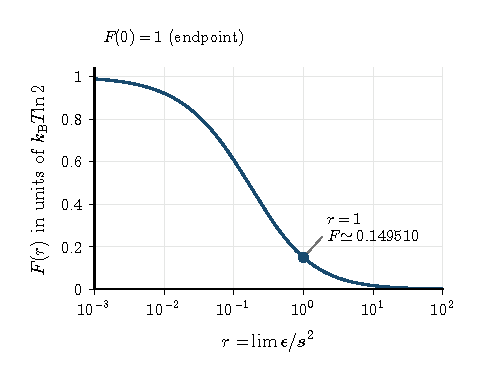
\includegraphics[width=8.5cm,height=6.4cm]{Graph/crossover.pdf}};
\node[align=center,font=\footnotesize,text=black!65] at (13.65,.12)
 {Positive error at every finite stage; finite $r$.};
\end{tikzpicture}%
}
 \caption{Conditional precision fixes a heat cost invisible to the average-state entropy decrease. (a) The targets have Bloch vectors $(-s,0,\pm c)$; the sideways displacement is enlarged for clarity. One fixed apparatus processes either input without a supplied label. Workspace return concerns its average marginal, while every reservoir component, including spent recovery qubits, is charged. (b) The optimal joint-limit heat $F(r)$ versus the finite limiting ratio $r=\lim\eps/s^2$. The horizontal axis is logarithmic; $r=0$ is an endpoint, not a plotted finite-ratio point. The marked value is $F(1)\simeq0.149510$. This is not a curve of finite-parameter optima. Figure code was prepared with AI assistance; the curve is evaluated from Eq.~\eqref{eq:limit}, not experimental data.}
 \label{fig:overview}
\end{figure*}

\para{Optimal precision--heat law}
Let $\qmin(s,\eps)$ be the infimum over all finite apparatuses satisfying Eqs.~\eqref{eq:task} and \eqref{eq:return}. For every sequence with $s\to0$, $\eps>0$, and $\eps/s^2\to r$ for a finite $r\ge0$,
\begin{equation}
 \qmin(s,\eps)\longrightarrow F(r)
 =\J\!\left(\frac1{\sqrt{1+4r}}\right).
 \label{eq:limit}
\end{equation}
In particular, $F(0)=1$, whereas $F(1)\simeq0.149510$ [Fig.~\ref{fig:overview}(b)]. Every finite stage has positive error. The result determines a joint limiting infimum, not an exact finite-$s$ optimum or a fixed-overlap zero-error limit. Each apparatus is finite, but the optimizing sequence may increase reservoir size, gaps, duration, and control complexity.

The squared-overlap scale has a geometric origin. The transverse displacement is $s$, but purity requires a longitudinal displacement $1-c=s^2/2+O(s^4)$. Errors much smaller than $s$ can still alter this second scale. Geometry identifies the relevant ratio; universality requires a bound on every allowed interaction.

\para{Precision forces an environmental record}
Write $E=AB$ and $\Omega=\tau_A\otimes\gamma_B$. For the system outputs define wrong-basis probabilities $\delta_0=\bra{1}\sigma_0\ket{1}$, $\delta_1=\bra{0}\sigma_1\ket{0}$ and coherences $z_x=\bra{0}\sigma_x\ket{1}$. The two trace-distance tests imply
\begin{equation}
 \begin{gathered}
 \bar\delta\equiv\frac{\delta_0+\delta_1}{2}\le d,\qquad |z_0+z_1|\ge s-2\eps,\\
 d=\frac{1-c}{2}+\eps .
 \end{gathered}
 \label{eq:kinematics}
\end{equation}
The first bound follows by measuring the wrong-basis event. The second follows because both target coherences equal $-s/2$. Accuracy therefore requires small transitions and a shared coherence simultaneously.

A complete cosine--sine decomposition~\cite{Sutton2008} parametrizes any joint unitary by environmental unitaries $V_0,V_1$ and a contraction $K$. It supplies comparison states $\tau_x=V_x\Omega V_x^\dagger$ and a coherence $\ell$ satisfying $|\ell-z_0-z_1|\le2\bar\delta$. No matrix block is inverted, so singular transitions and rank-deficient $\Omega$ are included. The replacement error is of order $d$, not $\sqrt d$; only the former is negligible relative to the order-$s$ signal in the crossover regime.

For complete eigenpairs $(p_i,u_i)$ and $(q_j,v_j)$ of $\tau_0,\tau_1$, set $w_{ij}=|\langle u_i|v_j\rangle|^2$. A weighted Cauchy--Schwarz inequality gives
\begin{equation}
 \begin{split}
 \Tcal&=\frac12\sum_{ij}\frac{(p_i-q_j)^2}{p_i+q_j}w_{ij},
 \qquad |\ell|^2\le4\bar\delta\Tcal,\\
 \Tcal&\ge b_0^2,\qquad
 b_0=\frac{[s-2\eps-2d]_+}{2\sqrt d},
 \end{split}
 \label{eq:spectral}
\end{equation}
where $[a]_+=\max\{0,a\}$ and zero-over-zero terms contribute zero. Thus suppressing unwanted transitions while maintaining the required coherence forces separation of the environmental comparison states.

This separation carries an information cost even when the states do not commute. Their equal-prior Holevo information, $\chi(\tau_0,\tau_1)=H((\tau_0+\tau_1)/2)-[H(\tau_0)+H(\tau_1)]/2$, obeys
\begin{equation}
 \chi(\tau_0,\tau_1)\ge\JS(P,Q)
 \ge\J(\sqrt{\Tcal})\ge\J(b_0),
 \label{eq:information}
\end{equation}
with algebraic distributions $P_{ij}=p_iw_{ij}$ and $Q_{ij}=q_jw_{ij}$. Here $\JS$ is Jensen--Shannon divergence in bits. Golden--Thompson~\cite{Golden1965,Thompson1965} yields the first inequality; the sharp scalar comparison~\cite{Nishiyama2022} yields the second. Commuting mirrored binary distributions saturate this information comparison. No simultaneous measurement of noncommuting eigenbases is assumed.

The comparison states need not be the physical outputs $E'_x$. Their mean trace distance is at most $f(d)=\sqrt{d(1-3d/4)}+d/2$. Attach a \emph{formal} binary label $\mathsf X$ and use $\chi(\mathsf X:E)=1-H(\mathsf X|E)$. Conditional-entropy continuity~\cite{Winter2016} then gives
\begin{equation}
 \chi(\mathsf X:E')\ge\J(b_0)-g(f(d)),
 \label{eq:physical-record}
\end{equation}
where $g(\eta)\to0$ as $\eta\to0$ and is specified in End Matter. Crucially, its dimension factor is that of the two-valued label, not the reservoir. Neither this label nor the purification used in the distance estimate is a supplied physical memory. This is what makes the converse uniform when apparatus dimensions grow.

\para{From information to heat}
On each branch, the total entropy is $H(\Omega)$. Subadditivity implies $H(E'_x)\ge H(\Omega)-H(\sigma_x)$. A qubit within trace distance $\eps<1/2$ of a pure state has entropy at most $h_2(\eps)$~\cite{Audenaert2007}. Averaging and adding the Holevo information gives $\Delta H_E\ge\chi(\mathsf X:E')-h_2(\eps)$. Independently, the initial averaged joint state has entropy $1+H(\Omega)$ and the final system has entropy at most one bit, hence $\Delta H_E\ge0$. Therefore
\begin{equation}
 \Delta H_E\ge L(s,\eps)
 =\max\{0,\J(b_0)-g(f(d))-h_2(\eps)\}.
 \label{eq:finite}
\end{equation}
This bound holds throughout $0<\eps<c/2$ and has no apparatus-dimension correction.

Only now does the Gibbs assumption enter. Its exact energy--entropy identity~\cite{ReebWolf2014} gives $q=\Delta H_B+\Db(\rho'_B\Vert\gamma_B)$, where $\Db$ is relative entropy in bits. Initial independence of $A,B$ yields
\begin{equation}
 q+\Delta H_A
 =\Delta H_E+I(A:B)'+\Db(\rho'_B\Vert\gamma_B)
 \ge L(s,\eps).
 \label{eq:ledger}
\end{equation}
Here $\Delta H_A=H(\rho'_A)-H(\tau_A)$ is an \emph{increase}; the two retained terms are nonnegative. Equation~\eqref{eq:return} sets $\Delta H_A=0$. The compulsory record concerns the complete environment $AB$, not necessarily the bath alone. Consuming clean workspace instead changes the resource balance. Approximate return has the dimension-dependent correction given in End Matter.

Along the limit in Eq.~\eqref{eq:limit}, $d/s^2\to1/4+r$, $b_0\to(1+4r)^{-1/2}$, and both finite corrections vanish. Equation~\eqref{eq:ledger} therefore bounds the infimum over all finite apparatuses from below by $F(r)$ in the limit.

\para{A matching thermal implementation}
The upper direction needs no workspace. Use one bath qubit of bias $b$, populations $(1\pm b)/2$, and gap $\beta\Delta=2\atanh b$. Choose
\begin{equation}
 \begin{split}
 u&=d,\quad \sin^2\theta=u,\quad b=\frac{s}{2\sqrt{u(1-u)}},\\
 U&=\mathrm{CNOT}_{S\to B}e^{i\theta X_S\otimes Y_B}.
 \end{split}
 \label{eq:collision}
\end{equation}
The domain $0<\eps<c/2$ ensures $0<b<1$: the bath is full rank and its gap finite. Direct calculation gives $\sigma_x=[I-sX+(-1)^x(c-2\eps)Z]/2$, so both errors equal $\eps$ and the transverse polarization is exact. The conditional bath states are $\gamma_b$ and $X\gamma_bX$; their average is $I/2$. The bare mean heat is $q_{\mathrm{bare}}=b\atanh b/\ln2$.

The spent working qubit is out of equilibrium. Successive thermal swaps~\cite{ReebWolf2014} recover its avoidable contribution without altering the system output. Add $M$ independent Gibbs qubits with biases $b_j=jb/M$ and gaps $\beta\Delta_j=2\atanh b_j$. Swap each with the working qubit in order. The working qubit returns to $\gamma_b$, but the spent qubits retain the energy changes and the first carries its earlier correlations. Charging the \emph{complete} reservoir gives
\begin{equation}
 \begin{split}
 q_M&=\frac{b}{M\ln2}\sum_{j=1}^M\atanh(jb/M),\\
 0&\le q_M-\J(b)\le\frac{b\atanh b}{M\ln2}.
 \end{split}
 \label{eq:recovery}
\end{equation}
The estimate follows from a right Riemann sum for $\int_0^b\atanh t\,\dd t=(\ln2)\J(b)$. Each positive-error stage has finite $b<1$, so a finite $M$ achieves any prescribed positive recovery residual. Choosing that residual to vanish gives the matching upper limit because $b\to(1+4r)^{-1/2}$. At $r=0$, gaps and recovery lengths can grow; no stage uses a pure Gibbs state.

\para{Consequences and a finite separation}
The same optimum controls the target channel $\Tcal_s(\rho)=\sum_x\bra{x}\rho\ket{x}\phi_x$. For half-diamond error, including reference-entangled inputs~\cite{Watrous2009},
\begin{equation}
 \qdiamond(s,\eps)=\qmin(s,\eps),
 \qquad 0<\eps<c/2.
 \label{eq:diamond}
\end{equation}
Full-channel accuracy implies the branch tests. Conversely, adding a zero-Hamiltonian Gibbs qubit to dephase the \emph{input} converts any branch-feasible apparatus at unchanged mean heat and workspace return. The converted channel's half-diamond error equals $\max_xD(\sigma_x,\phi_x)$. This proves equality of infima, not accuracy of an unmodified channel from two tests. Heat and return remain evaluated on the original equal-prior ensemble.

Exact outputs are different. At any fixed $0<s<1$, pure system outputs force product form with the environment. Unitarity would then require orthogonal environmental supports. Exact average workspace return confines both supports to $\supp\tau_A\otimes\Hcal_B$, while full bath rank and rank preservation force both to fill that same space. The contradiction excludes every finite exactly error-free apparatus, including rank-deficient workspace. Thus $F(0)$ is approached through positive errors, not attained by an exact finite implementation.

There is also a nonasymptotic separation. At $s=0.05$, Eq.~\eqref{eq:finite} gives $q\ge0.498044$ for $\eps=10^{-4}$. At the same overlap, the bare collision at $\eps=0.0025$ costs $q\simeq0.311485$. A strict universal lower bound exceeds a relaxed achievable cost, without recovery and without identifying either finite optimum. Complete derivations and deterministic consistency checks are provided in the appended technical sections below; the reproducible source is available at the pinned project revision~\cite{Repository}.

\para{Physical meaning}
For the bath-only construction, the heat identity separates into
\begin{equation}
 \begin{split}
 q&=\J(s)+I(S:B)'+\Db(\rho'_B\Vert\gamma_B),\\
 I(S:B)'&=\J(b)-\J(s).
 \end{split}
 \label{eq:cost-location}
\end{equation}
Reservoir-only recovery reduces disequilibrium while preserving its mutual information with $S$. Consequently, at $r=0$ the average entropy loss vanishes, the recoverable excess tends to zero, and the correlation contribution tends to one bit. This accounts for the surviving heat without violating the entropy bound or requiring final system--bath entanglement on the tested branches.

The result isolates conditional precision as a thermodynamic constraint: the same leading polarization can be reproduced exactly while the permitted near-purity error changes the optimal heat. The sharp law is for single-use mean reservoir heat, with driving and growing finite resources allowed. It is neither a collective work rate nor a platform power estimate. Its distinctive content is the positive-error, dimension-uniform crossover and its matching implementation, rather than operation-dependent dissipation alone.

\begin{acknowledgments}
The source project records AI assistance in the research and documentation. OpenAI ChatGPT (GPT-6 Astra Pro) assisted with preparation of this draft, literature comparison, LaTeX and figure code, and numerical consistency checks under the authors' editorial direction. The authors retain a record of the checks performed. This disclosure is provisional pending the authors' confirmation of the complete research-stage tool record and verification.
\end{acknowledgments}

\paragraph*{Data availability.}
No experimental data were generated. The formulas and finite computed examples underlying the figure and comparison are supplied with this manuscript and in the versioned project repository~\cite{Repository}.

% One references list for both the Letter and appended derivations.
%apsrev4-2.bst 2019-01-14 (MD) hand-edited version of apsrev4-1.bst
%Control: key (0)
%Control: author (8) initials jnrlst
%Control: editor formatted (1) identically to author
%Control: production of article title (0) allowed
%Control: page (0) single
%Control: year (1) truncated
%Control: production of eprint (0) enabled
\begin{thebibliography}{16}%
\makeatletter
\providecommand \@ifxundefined [1]{%
 \@ifx{#1\undefined}
}%
\providecommand \@ifnum [1]{%
 \ifnum #1\expandafter \@firstoftwo
 \else \expandafter \@secondoftwo
 \fi
}%
\providecommand \@ifx [1]{%
 \ifx #1\expandafter \@firstoftwo
 \else \expandafter \@secondoftwo
 \fi
}%
\providecommand \natexlab [1]{#1}%
\providecommand \enquote  [1]{``#1''}%
\providecommand \bibnamefont  [1]{#1}%
\providecommand \bibfnamefont [1]{#1}%
\providecommand \citenamefont [1]{#1}%
\providecommand \href@noop [0]{\@secondoftwo}%
\providecommand \href [0]{\begingroup \@sanitize@url \@href}%
\providecommand \@href[1]{\@@startlink{#1}\@@href}%
\providecommand \@@href[1]{\endgroup#1\@@endlink}%
\providecommand \@sanitize@url [0]{\catcode `\\12\catcode `\$12\catcode
  `\&12\catcode `\#12\catcode `\^12\catcode `\_12\catcode `\%12\relax}%
\providecommand \@@startlink[1]{}%
\providecommand \@@endlink[0]{}%
\providecommand \url  [0]{\begingroup\@sanitize@url \@url }%
\providecommand \@url [1]{\endgroup\@href {#1}{\urlprefix }}%
\providecommand \urlprefix  [0]{URL }%
\providecommand \Eprint [0]{\href }%
\providecommand \doibase [0]{https://doi.org/}%
\providecommand \selectlanguage [0]{\@gobble}%
\providecommand \bibinfo  [0]{\@secondoftwo}%
\providecommand \bibfield  [0]{\@secondoftwo}%
\providecommand \translation [1]{[#1]}%
\providecommand \BibitemOpen [0]{}%
\providecommand \bibitemStop [0]{}%
\providecommand \bibitemNoStop [0]{.\EOS\space}%
\providecommand \EOS [0]{\spacefactor3000\relax}%
\providecommand \BibitemShut  [1]{\csname bibitem#1\endcsname}%
\let\auto@bib@innerbib\@empty
%</preamble>
\bibitem [{\citenamefont {Landauer}(1961)}]{Landauer1961}%
  \BibitemOpen
  \bibfield  {author} {\bibinfo {author} {\bibfnamefont {R.}~\bibnamefont
  {Landauer}},\ }\bibfield  {title} {\bibinfo {title} {Irreversibility and heat
  generation in the computing process},\ }\href
  {https://doi.org/10.1147/rd.53.0183} {\bibfield  {journal} {\bibinfo
  {journal} {IBM J. Res. Dev.}\ }\textbf {\bibinfo {volume} {5}},\ \bibinfo
  {pages} {183} (\bibinfo {year} {1961})}\BibitemShut {NoStop}%
\bibitem [{\citenamefont {Reeb}\ and\ \citenamefont
  {Wolf}(2014)}]{ReebWolf2014}%
  \BibitemOpen
  \bibfield  {author} {\bibinfo {author} {\bibfnamefont {D.}~\bibnamefont
  {Reeb}}\ and\ \bibinfo {author} {\bibfnamefont {M.~M.}\ \bibnamefont
  {Wolf}},\ }\bibfield  {title} {\bibinfo {title} {An improved {Landauer}
  principle with finite-size corrections},\ }\href
  {https://doi.org/10.1088/1367-2630/16/10/103011} {\bibfield  {journal}
  {\bibinfo  {journal} {New J. Phys.}\ }\textbf {\bibinfo {volume} {16}},\
  \bibinfo {pages} {103011} (\bibinfo {year} {2014})},\ \Eprint
  {https://arxiv.org/abs/1306.4352} {arXiv:1306.4352} \BibitemShut {NoStop}%
\bibitem [{\citenamefont {Aksak}\ and\ \citenamefont
  {Turgut}(2011)}]{AksakTurgut2011}%
  \BibitemOpen
  \bibfield  {author} {\bibinfo {author} {\bibfnamefont {{\c{C}}.}~\bibnamefont
  {Aksak}}\ and\ \bibinfo {author} {\bibfnamefont {S.}~\bibnamefont {Turgut}},\
  }\bibfield  {title} {\bibinfo {title} {Heat transfer operators associated
  with quantum operations},\ }\href
  {https://doi.org/10.1088/1751-8113/44/27/275304} {\bibfield  {journal}
  {\bibinfo  {journal} {J. Phys. A: Math. Theor.}\ }\textbf {\bibinfo {volume}
  {44}},\ \bibinfo {pages} {275304} (\bibinfo {year} {2011})},\ \Eprint
  {https://arxiv.org/abs/1002.0733} {arXiv:1002.0733} \BibitemShut {NoStop}%
\bibitem [{\citenamefont {Bedingham}\ and\ \citenamefont
  {Maroney}(2016)}]{BedinghamMaroney2016}%
  \BibitemOpen
  \bibfield  {author} {\bibinfo {author} {\bibfnamefont {D.~J.}\ \bibnamefont
  {Bedingham}}\ and\ \bibinfo {author} {\bibfnamefont {O.~J.~E.}\ \bibnamefont
  {Maroney}},\ }\bibfield  {title} {\bibinfo {title} {The thermodynamic cost of
  quantum operations},\ }\href {https://doi.org/10.1088/1367-2630/18/11/113050}
  {\bibfield  {journal} {\bibinfo  {journal} {New J. Phys.}\ }\textbf {\bibinfo
  {volume} {18}},\ \bibinfo {pages} {113050} (\bibinfo {year} {2016})},\
  \Eprint {https://arxiv.org/abs/1604.03749} {arXiv:1604.03749} \BibitemShut
  {NoStop}%
\bibitem [{\citenamefont {Dunlop}\ \emph {et~al.}(2024)\citenamefont {Dunlop},
  \citenamefont {Cerisola}, \citenamefont {Tabanera-Bravo},\ and\ \citenamefont
  {Anders}}]{Dunlop2024}%
  \BibitemOpen
  \bibfield  {author} {\bibinfo {author} {\bibfnamefont {J.}~\bibnamefont
  {Dunlop}}, \bibinfo {author} {\bibfnamefont {F.}~\bibnamefont {Cerisola}},
  \bibinfo {author} {\bibfnamefont {J.}~\bibnamefont {Tabanera-Bravo}},\ and\
  \bibinfo {author} {\bibfnamefont {J.}~\bibnamefont {Anders}},\ }\bibfield
  {title} {\bibinfo {title} {Thermodynamically optimal protocols for
  dual-purpose qubit operations},\ }\href
  {https://doi.org/10.1103/PhysRevResearch.6.033005} {\bibfield  {journal}
  {\bibinfo  {journal} {Phys. Rev. Research}\ }\textbf {\bibinfo {volume}
  {6}},\ \bibinfo {pages} {033005} (\bibinfo {year} {2024})},\ \Eprint
  {https://arxiv.org/abs/2306.09088} {arXiv:2306.09088} \BibitemShut {NoStop}%
\bibitem [{\citenamefont {Chiribella}\ \emph {et~al.}(2022)\citenamefont
  {Chiribella}, \citenamefont {Meng}, \citenamefont {Renner},\ and\
  \citenamefont {Yung}}]{Chiribella2022}%
  \BibitemOpen
  \bibfield  {author} {\bibinfo {author} {\bibfnamefont {G.}~\bibnamefont
  {Chiribella}}, \bibinfo {author} {\bibfnamefont {F.}~\bibnamefont {Meng}},
  \bibinfo {author} {\bibfnamefont {R.}~\bibnamefont {Renner}},\ and\ \bibinfo
  {author} {\bibfnamefont {M.-H.}\ \bibnamefont {Yung}},\ }\bibfield  {title}
  {\bibinfo {title} {The nonequilibrium cost of accurate information
  processing},\ }\href {https://doi.org/10.1038/s41467-022-34541-w} {\bibfield
  {journal} {\bibinfo  {journal} {Nat. Commun.}\ }\textbf {\bibinfo {volume}
  {13}},\ \bibinfo {pages} {7155} (\bibinfo {year} {2022})},\ \Eprint
  {https://arxiv.org/abs/2203.09369} {arXiv:2203.09369} \BibitemShut {NoStop}%
\bibitem [{\citenamefont {Faist}\ and\ \citenamefont
  {Renner}(2018)}]{FaistRenner2018}%
  \BibitemOpen
  \bibfield  {author} {\bibinfo {author} {\bibfnamefont {P.}~\bibnamefont
  {Faist}}\ and\ \bibinfo {author} {\bibfnamefont {R.}~\bibnamefont {Renner}},\
  }\bibfield  {title} {\bibinfo {title} {Fundamental work cost of quantum
  processes},\ }\href {https://doi.org/10.1103/PhysRevX.8.021011} {\bibfield
  {journal} {\bibinfo  {journal} {Phys. Rev. X}\ }\textbf {\bibinfo {volume}
  {8}},\ \bibinfo {pages} {021011} (\bibinfo {year} {2018})},\ \Eprint
  {https://arxiv.org/abs/1709.00506} {arXiv:1709.00506} \BibitemShut {NoStop}%
\bibitem [{\citenamefont {Faist}\ \emph {et~al.}(2019)\citenamefont {Faist},
  \citenamefont {Berta},\ and\ \citenamefont
  {Brand{\~a}o}}]{FaistBertaBrandao2019}%
  \BibitemOpen
  \bibfield  {author} {\bibinfo {author} {\bibfnamefont {P.}~\bibnamefont
  {Faist}}, \bibinfo {author} {\bibfnamefont {M.}~\bibnamefont {Berta}},\ and\
  \bibinfo {author} {\bibfnamefont {F.}~\bibnamefont {Brand{\~a}o}},\
  }\bibfield  {title} {\bibinfo {title} {Thermodynamic capacity of quantum
  processes},\ }\href {https://doi.org/10.1103/PhysRevLett.122.200601}
  {\bibfield  {journal} {\bibinfo  {journal} {Phys. Rev. Lett.}\ }\textbf
  {\bibinfo {volume} {122}},\ \bibinfo {pages} {200601} (\bibinfo {year}
  {2019})},\ \Eprint {https://arxiv.org/abs/1807.05610} {arXiv:1807.05610}
  \BibitemShut {NoStop}%
\bibitem [{\citenamefont {Sutton}(2008)}]{Sutton2008}%
  \BibitemOpen
  \bibfield  {author} {\bibinfo {author} {\bibfnamefont {B.~D.}\ \bibnamefont
  {Sutton}},\ }\href@noop {} {\bibinfo {title} {Computing the complete {CS}
  decomposition}} (\bibinfo {year} {2008}),\ \Eprint
  {https://arxiv.org/abs/0707.1838v3} {arXiv:0707.1838v3 [math.NA]}
  \BibitemShut {NoStop}%
\bibitem [{\citenamefont {Golden}(1965)}]{Golden1965}%
  \BibitemOpen
  \bibfield  {author} {\bibinfo {author} {\bibfnamefont {S.}~\bibnamefont
  {Golden}},\ }\bibfield  {title} {\bibinfo {title} {Lower bounds for the
  {Helmholtz} function},\ }\href {https://doi.org/10.1103/PhysRev.137.B1127}
  {\bibfield  {journal} {\bibinfo  {journal} {Phys. Rev.}\ }\textbf {\bibinfo
  {volume} {137}},\ \bibinfo {pages} {B1127} (\bibinfo {year}
  {1965})}\BibitemShut {NoStop}%
\bibitem [{\citenamefont {Thompson}(1965)}]{Thompson1965}%
  \BibitemOpen
  \bibfield  {author} {\bibinfo {author} {\bibfnamefont {C.~J.}\ \bibnamefont
  {Thompson}},\ }\bibfield  {title} {\bibinfo {title} {Inequality with
  applications in statistical mechanics},\ }\href@noop {} {\bibfield  {journal}
  {\bibinfo  {journal} {J. Math. Phys.}\ }\textbf {\bibinfo {volume} {6}},\
  \bibinfo {pages} {1812} (\bibinfo {year} {1965})}\BibitemShut {NoStop}%
\bibitem [{\citenamefont {Nishiyama}(2022)}]{Nishiyama2022}%
  \BibitemOpen
  \bibfield  {author} {\bibinfo {author} {\bibfnamefont {T.}~\bibnamefont
  {Nishiyama}},\ }\href@noop {} {\bibinfo {title} {On relations between tight
  bounds for symmetric $f$-divergences and binary divergences}} (\bibinfo
  {year} {2022}),\ \Eprint {https://arxiv.org/abs/2210.09571v2}
  {arXiv:2210.09571v2 [cs.IT]} \BibitemShut {NoStop}%
\bibitem [{\citenamefont {Winter}(2016)}]{Winter2016}%
  \BibitemOpen
  \bibfield  {author} {\bibinfo {author} {\bibfnamefont {A.}~\bibnamefont
  {Winter}},\ }\bibfield  {title} {\bibinfo {title} {Tight uniform continuity
  bounds for quantum entropies: conditional entropy, relative entropy distance
  and energy constraints},\ }\href {https://doi.org/10.1007/s00220-016-2609-8}
  {\bibfield  {journal} {\bibinfo  {journal} {Commun. Math. Phys.}\ }\textbf
  {\bibinfo {volume} {347}},\ \bibinfo {pages} {291} (\bibinfo {year}
  {2016})},\ \Eprint {https://arxiv.org/abs/1507.07775} {arXiv:1507.07775}
  \BibitemShut {NoStop}%
\bibitem [{\citenamefont {Audenaert}(2007)}]{Audenaert2007}%
  \BibitemOpen
  \bibfield  {author} {\bibinfo {author} {\bibfnamefont {K.~M.~R.}\
  \bibnamefont {Audenaert}},\ }\bibfield  {title} {\bibinfo {title} {A sharp
  continuity estimate for the von {Neumann} entropy},\ }\href
  {https://doi.org/10.1088/1751-8113/40/28/S18} {\bibfield  {journal} {\bibinfo
   {journal} {J. Phys. A: Math. Theor.}\ }\textbf {\bibinfo {volume} {40}},\
  \bibinfo {pages} {8127} (\bibinfo {year} {2007})},\ \Eprint
  {https://arxiv.org/abs/quant-ph/0610146} {arXiv:quant-ph/0610146}
  \BibitemShut {NoStop}%
\bibitem [{\citenamefont {Watrous}(2009)}]{Watrous2009}%
  \BibitemOpen
  \bibfield  {author} {\bibinfo {author} {\bibfnamefont {J.}~\bibnamefont
  {Watrous}},\ }\bibfield  {title} {\bibinfo {title} {Semidefinite programs for
  completely bounded norms},\ }\href
  {https://doi.org/10.4086/toc.2009.v005a011} {\bibfield  {journal} {\bibinfo
  {journal} {Theory Comput.}\ }\textbf {\bibinfo {volume} {5}},\ \bibinfo
  {pages} {217} (\bibinfo {year} {2009})},\ \Eprint
  {https://arxiv.org/abs/0901.4709} {arXiv:0901.4709} \BibitemShut {NoStop}%
\bibitem [{\citenamefont {Lin}(2026)}]{Repository}%
  \BibitemOpen
  \bibfield  {author} {\bibinfo {author} {\bibfnamefont {R.}~\bibnamefont
  {Lin}},\ }\href@noop {} {\bibinfo {title} {Quantum-precision-heat-tradeoff:
  scientific account and reproducible calculations}},\ \bibinfo {howpublished}
  {\href{https://github.com/GoGoKo699/Quantum-Precision-Heat-Tradeoff/tree/f749753c5000bfa3efb3466d67c12b4b1befbb4b}{Versioned
  scientific repository}} (\bibinfo {year} {2026}),\ \bibinfo {note} {revision
  \texttt{f749753c5000}, accessed October 21, 2026}\BibitemShut {NoStop}%
\end{thebibliography}%

\onecolumngrid
\clearpage
\twocolumngrid
\renewcommand{\theHsection}{endmatter.\arabic{section}}
\renewcommand{\theHsubsection}{endmatter.\arabic{section}.\arabic{subsection}}
% End Matter: specialist details; compiled after the references.
\setcounter{section}{0}
\setcounter{secnumdepth}{1}
\renewcommand{\thesection}{\Alph{section}}
\setcounter{equation}{0}
\renewcommand{\theequation}{E\arabic{equation}}
\renewcommand{\theHequation}{endmatter.\arabic{equation}}
\begin{center}\textbf{END MATTER}\end{center}
\section{Finite corrections and workspace return}
For $0<s<1$ and $0<\eps<c/2$, $d=(1-c)/2+\eps<1/2$. With $b_0$ from Eq.~\eqref{eq:spectral}, define
\begin{align}
 f(d)&=\sqrt{d(1-3d/4)}+d/2,\nonumber\\
 g(\eta)&=\min\!\left\{1,\eta+(1+\eta)
 h_2\!\left(\frac{\eta}{1+\eta}\right)\right\}.
 \label{eq:E-corrections}
\end{align}
Gibbs accounting gives
\begin{equation}
 q+\Delta H_A\ge L(s,\eps)+I(A:B)'
                  +\Db(\rho'_B\Vert\gamma_B).
 \label{eq:E-strong}
\end{equation}
For an $n$-dimensional workspace returned within trace distance $\delta$, put $t=\min\{\delta,1-1/n\}$ and
\begin{equation}
 \begin{gathered}
 a_n(\delta)=h_2(t)+t\log_2(n-1),\\
 q\ge L(s,\eps)-a_n(\delta).
 \end{gathered}
 \label{eq:E-approx-return}
\end{equation}
For $n=1$ set $a_1=0$. The entropy-continuity bound~\cite{Audenaert2007} gives $\Delta H_A\le a_n$. Do not clip a negative bound to zero: consumed workspace supplies entropy capacity. The limiting converse survives a uniformly vanishing allowance, including fixed $n$ and $\delta\to0$.

\section{The dimension-uniform information bridge}
The complete cosine--sine decomposition~\cite{Sutton2008} gives
\begin{equation}
 U=\begin{pmatrix}V_0C_0&-V_0K^\dagger\\V_1K&V_1C_1\end{pmatrix},
 \quad
 \begin{matrix}C_0=\sqrt{I-K^\dagger K},\\C_1=\sqrt{I-KK^\dagger}.\end{matrix}
 \label{eq:E-CS}
\end{equation}
With $\tau_x=V_x\Omega V_x^\dagger$, $T_E=V_1KV_0^\dagger$, and $\ell=\Tr[(\tau_0-\tau_1)T_E^\dagger]$, the probabilities are $\delta_0=\Tr(\tau_0T_E^\dagger T_E)$ and $\delta_1=\Tr(\tau_1T_ET_E^\dagger)$. Replacing $C_x$ by $I$ in the coherences gives $\ell$. Cauchy--Schwarz and $(I-C_x)^2\le I-C_x^2$ bound each error by $\delta_x$, including singular blocks and rank-deficient $\Omega$.

In the mixed eigenbases, weighted Cauchy--Schwarz has factors $2\Tcal$ and $2\bar\delta$, proving Eq.~\eqref{eq:spectral} even with zero eigenvalues. For Eq.~\eqref{eq:information}, put $M=(\tau_0+\tau_1)/2$ and $m_{ij}=(p_i+q_j)/2$. Golden--Thompson implies
\begin{equation}
 \Tr e^{-tM}\le\sum_{ij}w_{ij}e^{-tm_{ij}},\qquad t>0.
 \label{eq:E-GT}
\end{equation}
Integrating with a positive $t^{-2}$ weight after subtracting the common affine terms in the representation of $x\ln x$ gives
\begin{equation}
 \Tr(M\ln M)\le\sum_{ij}w_{ij}m_{ij}\ln m_{ij}.
 \label{eq:E-entropy-comparison}
\end{equation}
This gives the direction $\chi\ge\JS(P,Q)$. On positive-weight cells define $\mu_{ij}=(P_{ij}+Q_{ij})/2$ and $a_{ij}=(P_{ij}-Q_{ij})/(P_{ij}+Q_{ij})$. Then $\JS=\sum\mu_{ij}\J(a_{ij})$ and $\Tcal=\sum\mu_{ij}a_{ij}^2$. Convexity of $t\mapsto\J(\sqrt t)$ gives the sharp scalar bound~\cite{Nishiyama2022}. Mirrored binary distributions with bias $b$ attain $\Tcal=b^2$ and $\JS=\J(b)$. This need not saturate the finite kinematic estimates.

To transfer to actual outputs, purify $\Omega$ only for a distance estimate. Let $v$ be the comparison purification in the appropriate $V_x$ frame and $a=(C_x\otimes I)v$. Then $\norm{a}^2=1-\delta_x$ and $\langle v|a\rangle\ge1-\delta_x$. The rank-one trace-norm identity and the failed branch of trace $\delta_x$ give
\begin{equation}
 D(E'_x,\tau_x)\le f(\delta_x),\qquad
 \frac12\sum_xD(E'_x,\tau_x)\le f(d).
 \label{eq:E-disturbance}
\end{equation}
For the resulting classical--quantum states, the improved conditional-entropy continuity bound~\cite{Winter2016} involves $\log_2\dim\mathsf X=1$, not $\dim E$. Since $0\le H(\mathsf X|E)\le1$, the correction can also be capped at one. This yields exactly $g(f(d))$. 

\section{Operational consequences}
For any branch-feasible device add a Gibbs qubit $C$ with $H_C=0$ and state $I_C/2$. Apply the controlled phase $W_{CS}=\proj{0}_C\otimes I_S+\proj{1}_C\otimes Z_S$ before the original unitary. Each basis-input joint state is unchanged and $C$ has zero energy, preserving all charged branch energy changes and average workspace return. For general inputs the system channel becomes $\widetilde\Ncal=\Ncal\circ\Dcal_Z$.

Let $\Delta_x=\sigma_x-\phi_x$. For any state $\rho_{SR}$ with a reference, its positive diagonal blocks $R_x=\bra{x}\rho_{SR}\ket{x}$ have total trace one. Hence
\begin{equation}
 \frac12\left\|\sum_x\Delta_x\otimes R_x\right\|_1
 \le\max_x\frac{\norm{\Delta_x}_1}{2}.
 \label{eq:E-channel}
\end{equation}
A maximizing basis input gives equality. Trace-norm contractivity of pinching extends this to arbitrary operators, establishing the diamond bound. Both directions of the infimum comparison give Eq.~\eqref{eq:diamond}. Adding $C$ is allowed because reservoir dimension is not capped.

For the exact-output obstruction let $k=\rank\tau_A$ and $d_B=\dim\Hcal_B$. Purity forces $\rho'_{SAB,x}=\phi_x\otimes\omega_x$ with $\rank\omega_x=kd_B$. Positivity and Eq.~\eqref{eq:return} prohibit support outside $\mathcal K=\supp\tau_A\otimes\Hcal_B$. Thus both $\omega_x$ are strictly positive on the same $kd_B$-dimensional space, and $\Tr(\omega_0\omega_1)>0$. Yet preserved orthogonality requires
\begin{equation}
 0=\Tr(\rho'_{SAB,0}\rho'_{SAB,1})
   =s^2\Tr(\omega_0\omega_1)>0,
 \label{eq:E-rank}
\end{equation}
a contradiction. Only average marginal return was used; conditional return and decorrelation were not assumed.


% The detailed derivations are part of this arXiv article rather than a second PDF.
\clearpage
\onecolumngrid
\clearpage
\setcounter{section}{0}
\setcounter{subsection}{0}
\setcounter{equation}{0}
\setcounter{secnumdepth}{2}
\renewcommand{\thesection}{S\Roman{section}}
\renewcommand{\theHsection}{arxivsupp.\arabic{section}}
\renewcommand{\theHsubsection}{arxivsupp.\arabic{section}.\arabic{subsection}}
\renewcommand{\theequation}{S\arabic{equation}}
\renewcommand{\theHequation}{arxivsupp.\arabic{equation}}
\begin{center}
 {\large\bfseries DETAILED DERIVATIONS AND SUPPORTING RESULTS}
\end{center}
\vspace{0.8em}
% Keep the long technical appendix readable as a single-column article.
\fontsize{10}{13}\selectfont
\setlength{\parskip}{1.5pt}
\section{Statement, conventions, and resource boundary}
\label{sec:conventions}
These sections give the complete argument supporting the Letter. Every system is finite dimensional. The input qubit $S$ is prepared in $\ket{x}$, $x=0,1$, with equal probabilities. The workspace $A$ starts in a fixed state $\tau_A$, and the complete reservoir $B$ starts in $\gamma_B=e^{-\beta H_B}/\Tr e^{-\beta H_B}$, where $\beta=(\kb T)^{-1}$, $T>0$, and all energy levels are finite. The three systems are initially independent. One fixed unitary $U$ acts on $SAB$, without a separate supplied input label. Predetermined driving is permitted. Fresh Gibbs systems used during recovery belong to $B$ from the beginning; their final energy changes are charged even after they are no longer accessed.

Write $E=AB$ and $\Omega=\tau_A\otimes\gamma_B$. The workspace can be nonthermal or rank deficient. No Gibbs property of $\Omega$ is assumed in the kinematic or information arguments. It enters only through the actual reservoir factor in the heat identity. For $0<s<1$, put $c=\sqrt{1-s^2}$ and
\begin{equation}
 \phi_x=\frac{I-sX+(-1)^xcZ}{2},\qquad
 \sigma_x=\Tr_E U(\proj{x}\otimes\Omega)U^\dagger,
 \qquad D(\sigma_x,\phi_x)\le\eps\quad(x=0,1).
 \label{eq:S-task}
\end{equation}
Here $X,Y,Z$ are Pauli matrices; $\phi_x$ denotes a density operator, whereas $\ket{\phi_x}$ denotes a normalized vector representing that pure state. Its overlap obeys $|\langle\phi_0|\phi_1\rangle|=s$. The trace distance is $D(\rho,\sigma)=\norm{\rho-\sigma}_1/2$, with $\norm{M}_1=\Tr\sqrt{M^\dagger M}$. Unless explicitly marked otherwise, entropies use base-two logarithms:
\begin{align}
 H(\rho)&=-\Tr\rho\log_2\rho,&
 h_2(p)&=-p\log_2p-(1-p)\log_2(1-p),\nonumber\\
 \Db(\rho\Vert\sigma)&=\Tr\rho(\log_2\rho-\log_2\sigma),&
 \J(b)&=1-h_2\!\left(\frac{1+b}{2}\right).
 \label{eq:S-entropies}
\end{align}
The convention is $0\log 0=0$. Relative entropy is infinite unless the first support lies within the second. The Gibbs denominator is full rank. A prime indicates a final state; an unconditioned final marginal is averaged over $x$. Define
\begin{equation}
 Q=\Tr H_B(\rho'_B-\gamma_B),\quad
 q=\frac{\beta Q}{\ln2},\quad
 \Delta H_A=H(\rho'_A)-H(\tau_A),\quad
 \Delta H_E=H(\rho'_E)-H(\Omega).
 \label{eq:S-cost}
\end{equation}
Positive $Q$ means that the complete reservoir gains mean energy. The optimization requires $\rho'_A=(\rho'_{A,0}+\rho'_{A,1})/2=\tau_A$, not conditional return or final decorrelation. A returned marginal alone does not establish independent reuse with arbitrarily correlated later inputs. With zero system boundary Hamiltonian, unchanged workspace and reservoir Hamiltonians, and interactions off at the boundaries, net supplied work is $W=Q+\Delta E_A$. Exact marginal return gives $W=Q$. This does not identify arbitrary battery-work costs with reservoir heat. Preparation of the source and construction of the controller are outside the model.

For $0<\eps<c/2$, define
\begin{align}
 d&=\frac{1-c}{2}+\eps=\frac{s^2}{2(1+c)}+\eps,
 & b_0&=\frac{[s-2\eps-2d]_+}{2\sqrt d},\nonumber\\
 f(d)&=\sqrt{d(1-3d/4)}+\frac d2,
 & g(\eta)&=\min\!\left\{1,\eta+(1+\eta)h_2\!\left(\frac{\eta}{1+\eta}\right)\right\},\nonumber\\
 L(s,\eps)&=\max\{0,\J(b_0)-g(f(d))-h_2(\eps)\}.&&
 \label{eq:S-finite-def}
\end{align}
Here $[a]_+=\max\{0,a\}$. The domain gives $0<d<1/2$ and $0\le b_0<1$. We prove
\begin{equation}
 q+\Delta H_A\ge L(s,\eps)+I(A:B)'+\Db(\rho'_B\Vert\gamma_B)\ge L(s,\eps).
 \label{eq:S-finite-thm}
\end{equation}
The bound has no workspace or bath dimension factor. Its finite value is not asserted to be optimal. If $\qmin$ is the infimum under exact ensemble-average workspace return, the matching construction proves, for every sequence $s\to0$, $\eps>0$, $\eps/s^2\to r<\infty$,
\begin{equation}
 \qmin(s,\eps)\longrightarrow
 F(r)=\J\!\left((1+4r)^{-1/2}\right),\qquad r\ge0.
 \label{eq:S-limit}
\end{equation}
No uniform upper bound on finite apparatus size, energy gaps, duration, or control complexity is imposed.

\section{Conditional accuracy gives two kinematic constraints}
\label{sec:output}
Let $\delta_0=\bra1\sigma_0\ket1$, $\delta_1=\bra0\sigma_1\ket0$ be the wrong-basis probabilities and let $z_x=\bra0\sigma_x\ket1$ be the coherences. Both targets have wrong-basis probability $(1-c)/2$. Trace distance bounds the change of any measurement-event probability, so $\delta_x\le d$ and $\bar\delta=(\delta_0+\delta_1)/2\le d$.

For the Hermitian traceless difference between two qubit states, write
\begin{equation}
 M=\begin{pmatrix}a&z\\z^*&-a\end{pmatrix},\qquad
 \frac12\norm M_1=\sqrt{a^2+|z|^2}.
 \label{eq:S-qubit-distance}
\end{equation}
Each target off-diagonal entry is $-s/2$. Equation~\eqref{eq:S-task} therefore gives $|z_x+s/2|\le\eps$. Summing and applying the triangle inequality yields
\begin{equation}
 \bar\delta\le d,\qquad |z_0+z_1|\ge s-2\eps.
 \label{eq:S-output-constraints}
\end{equation}
These are necessary conditions on each accurate apparatus. Matching the mean state or only the wrong-basis populations would not suffice.

\section{Complete unitary reduction and the coherence error}
\label{sec:CS}
Regard $U$ as a two-by-two block matrix in the system basis, with all blocks acting on $E$. The complete cosine--sine decomposition~\cite{Sutton2008} writes it as block-diagonal unitary factors surrounding
\begin{equation}
 \begin{pmatrix}\Gamma&-\Lambda\\\Lambda&\Gamma\end{pmatrix},\qquad
 \Gamma=\operatorname{diag}(\cos\theta_j),\quad
 \Lambda=\operatorname{diag}(\sin\theta_j),\quad 0\le\theta_j\le\frac\pi2.
 \label{eq:S-CS-central}
\end{equation}
Let the outside unitary blocks be $L_i,R_i$ so that $U=\operatorname{diag}(L_0,L_1)\mathsf C\operatorname{diag}(R_0^\dagger,R_1^\dagger)$. Set $V_i=L_iR_i^\dagger$ and $K=R_1\Lambda R_0^\dagger$. Then
\begin{equation}
 U=\begin{pmatrix}V_0C_0&-V_0K^\dagger\\V_1K&V_1C_1\end{pmatrix},
 \qquad C_0=\sqrt{I-K^\dagger K},\quad C_1=\sqrt{I-KK^\dagger}.
 \label{eq:S-CS}
\end{equation}
The transition operator $K$ is a contraction. Endpoint angles include singular values zero and one. No inverse of a survival or transition block is used, and $\Omega$ need not have full rank.

Define the comparison states $\tau_i=V_i\Omega V_i^\dagger$, the operator $T_E=V_1KV_0^\dagger$, and
\begin{equation}
 \ell=\Tr[(\tau_0-\tau_1)T_E^\dagger],\qquad
 \delta_0=\Tr(\tau_0T_E^\dagger T_E),\quad
 \delta_1=\Tr(\tau_1T_ET_E^\dagger).
 \label{eq:S-comparison}
\end{equation}
The subscript on $T_E$ distinguishes this transition operator from temperature. The comparison states are not generally the actual environmental outputs.

The two output coherences obtained directly from Eq.~\eqref{eq:S-CS} are
\begin{equation}
 z_0=\Tr(V_0C_0\Omega K^\dagger V_1^\dagger),\qquad
 z_1=-\Tr(V_0K^\dagger\Omega C_1V_1^\dagger).
 \label{eq:S-z}
\end{equation}
Replacing $C_0,C_1$ by the identity makes their sum exactly $\ell$. To control this replacement, set $W_E=V_1^\dagger V_0$. The first error is
\begin{align}
 |\Tr[\Omega K^\dagger W_E(I-C_0)]|^2
 &\le\Tr(\Omega K^\dagger K)\Tr[\Omega(I-C_0)^2]
 \le\delta_0^2.
 \label{eq:S-orderd}
\end{align}
The first step is weighted Hilbert--Schmidt Cauchy--Schwarz, with $W_E$ unitary. The second uses $(I-C_0)^2\le I-C_0^2=K^\dagger K$. Writing the second error as $\Tr[\Omega(I-C_1)W_EK^\dagger]$ gives the corresponding bound $\delta_1$. Consequently,
\begin{equation}
 |\ell-z_0-z_1|\le\delta_0+\delta_1,
 \qquad |\ell|\ge[s-2\eps-2d]_+.
 \label{eq:S-ell}
\end{equation}
The order-$d$ error is essential: when $d$ is of order $s^2$, an order-$\sqrt d$ estimate could erase the leading order-$s$ coherence constraint.

\section{Spectral discrimination forced by the coherence}
\label{sec:spectral}
Choose complete eigenpairs $(p_i,u_i)$ and $(q_j,v_j)$ for $\tau_0,\tau_1$, including zero eigenvalues, and set
\begin{equation}
 w_{ij}=|\langle u_i|v_j\rangle|^2,\qquad
 \Tcal=\frac12\sum_{ij}\frac{(p_i-q_j)^2}{p_i+q_j}w_{ij}.
 \label{eq:S-triangular}
\end{equation}
A term with $p_i=q_j=0$ is defined to be zero. Both the row and column sums of $w$ equal one. Since $(p-q)^2\le(p+q)^2$, the normalization gives $0\le\Tcal\le1$.

Put $t_{ij}=\bra{u_i}T_E^\dagger\ket{v_j}$. Inserting the complete eigenbases gives
\begin{align}
 \ell&=\sum_{ij}(p_i-q_j)\langle v_j|u_i\rangle t_{ij},\nonumber\\
 \sum_{ij}(p_i+q_j)|t_{ij}|^2
 &=\Tr(\tau_0T_E^\dagger T_E)+\Tr(\tau_1T_ET_E^\dagger)=2\bar\delta.
 \label{eq:S-weighted}
\end{align}
Weighted Cauchy--Schwarz therefore yields
\begin{equation}
 |\ell|^2\le (2\Tcal)(2\bar\delta)\le4d\Tcal,
 \qquad \Tcal\ge b_0^2.
 \label{eq:S-separation}
\end{equation}
Zero-denominator cells have zero numerator and contribute nothing to this step. The proof uses the particular mixed-eigenbasis expression in Eq.~\eqref{eq:S-triangular}; an arbitrary quantum divergence with the same commuting specialization cannot be substituted without a separate argument.

\section{The noncommuting spectral-to-information comparison}
\label{sec:information}
For equally likely states define $\chi(\tau_0,\tau_1)=H(M)-[H(\tau_0)+H(\tau_1)]/2$, where $M=(\tau_0+\tau_1)/2$. Set $P_{ij}=p_iw_{ij}$ and $Q_{ij}=q_jw_{ij}$. They are normalized classical distributions, but no measurement that simultaneously reveals both eigenbases is asserted. Their Jensen--Shannon divergence is
\begin{equation}
 \JS(P,Q)=\frac12\sum_{ij}P_{ij}\log_2\frac{2P_{ij}}{P_{ij}+Q_{ij}}
          +\frac12\sum_{ij}Q_{ij}\log_2\frac{2Q_{ij}}{P_{ij}+Q_{ij}}.
 \label{eq:S-JS}
\end{equation}
Zero-weight contributions vanish by continuity. We establish the direction
\begin{equation}
 \chi(\tau_0,\tau_1)\ge\JS(P,Q)\ge\J(\sqrt{\Tcal}).
 \label{eq:S-info-chain}
\end{equation}

\subsection{Quantum entropy versus the algebraic distributions}
Work in natural logarithms in this subsection only. Define $m_{ij}=(p_i+q_j)/2$ and $A_0=(\sum_i p_i\ln p_i+\sum_jq_j\ln q_j)/2$. Direct expansion gives
\begin{equation}
 (\ln2)\chi=A_0-\Tr(M\ln M),\qquad
 (\ln2)\JS=A_0-\sum_{ij}w_{ij}m_{ij}\ln m_{ij}.
 \label{eq:S-entropy-expansion}
\end{equation}
The Golden--Thompson inequality~\cite{Golden1965,Thompson1965} implies, for $t>0$,
\begin{equation}
 \Tr e^{-tM}\le\Tr(e^{-t\tau_0/2}e^{-t\tau_1/2})
 =\sum_{ij}w_{ij}e^{-tm_{ij}}.
 \label{eq:S-GT}
\end{equation}
To pass from this trace inequality to entropy, use
\begin{equation}
 R_t(x)=e^{-tx}-e^{-t}+(x-1)t e^{-t},\qquad
 x\ln x=x-1+\int_0^\infty\frac{R_t(x)}{t^2}\,\dd t.
 \label{eq:S-integral}
\end{equation}
For $x>0$, differentiating the integral twice gives $1/x$; the integral and its first derivative vanish at $x=1$. The affine term then supplies the value and derivative of $x\ln x$. Convexity of the exponential gives $R_t(x)\ge0$.

Apply Eq.~\eqref{eq:S-integral} to the eigenvalues of $M$ and to $m_{ij}$ with weights $w_{ij}$. The constant and linear terms cancel: $\sum_{ij}w_{ij}=\dim E$ and $\sum_{ij}w_{ij}m_{ij}=\Tr M=1$. Integrating Eq.~\eqref{eq:S-GT} with the positive weight $t^{-2}$ gives
\begin{equation}
 \Tr(M\ln M)\le\sum_{ij}w_{ij}m_{ij}\ln m_{ij}.
 \label{eq:S-GT-entropy}
\end{equation}
Substitution into Eq.~\eqref{eq:S-entropy-expansion} proves $\chi\ge\JS$, not the reverse. For zero eigenvalues, mix both states with the same maximally mixed state, use complete eigenbases, and take the mixing weight to zero. Continuity of $x\ln x$ at zero closes the finite-dimensional argument.

\subsection{Sharp scalar comparison}
On cells with $P_{ij}+Q_{ij}>0$, write
\begin{equation}
 \mu_{ij}=\frac{P_{ij}+Q_{ij}}2,\qquad
 a_{ij}=\frac{P_{ij}-Q_{ij}}{P_{ij}+Q_{ij}}.
 \label{eq:S-mua}
\end{equation}
Then $\sum\mu_{ij}=1$, $|a_{ij}|\le1$, and
\begin{equation}
 \JS(P,Q)=\sum_{ij}\mu_{ij}\J(a_{ij}),\qquad
 \Tcal=\sum_{ij}\mu_{ij}a_{ij}^2.
 \label{eq:S-moments}
\end{equation}
The function $\J$ is even. Its expansion
\begin{equation}
 \J(a)=\frac1{\ln2}\sum_{k=1}^{\infty}
             \frac{a^{2k}}{(2k)(2k-1)}
 \label{eq:S-series}
\end{equation}
shows that $t\mapsto\J(\sqrt t)$ is convex on $[0,1]$, with endpoint values by continuity. Jensen's inequality proves the second step of Eq.~\eqref{eq:S-info-chain}. This is the sharp scalar Jensen--Shannon/triangular-discrimination comparison of Ref.~\cite{Nishiyama2022}, with the same factor of one half in the definition of triangular discrimination. Mirrored binary distributions
\begin{equation}
 P=\left(\frac{1+b}{2},\frac{1-b}{2}\right),\qquad
 Q=\left(\frac{1-b}{2},\frac{1+b}{2}\right)
 \label{eq:S-mirrored}
\end{equation}
attain $\Tcal=b^2$ and $\JS=\J(b)$. Commuting density operators with these populations also attain the quantum comparison. This does not assert equality in the earlier finite kinematic estimates. Combining with Eq.~\eqref{eq:S-separation} gives $\chi(\tau_0,\tau_1)\ge\J(b_0)$.

\section{Transfer to the physical environment without a size penalty}
\label{sec:transfer}
Let $E'_x$ denote the actual conditional environment state after $U$. A purification of $\Omega$ is used here solely to estimate a norm. It is not a physically accessible auxiliary and supplies no entropy or energy resource.

For branch $x$, work in its survival frame $V_x$. Let $v$ be a unit vector purifying the comparison state in that frame and let $a=(C_x\otimes I)v$ be the unnormalized survival vector. With $\delta=\delta_x$,
\begin{equation}
 \langle a|a\rangle=1-\delta,\qquad
 \langle v|a\rangle\ge1-\delta.
 \label{eq:S-survival}
\end{equation}
The second inequality follows from $0\le C_x\le I$ and $C_x\ge C_x^2$. The two-dimensional rank-one trace-norm identity gives
\begin{equation}
 \bigl\|\proj{v}-\proj{a}\bigr\|_1^2
 =(2-\delta)^2-4|\langle v|a\rangle|^2
 \le4\delta-3\delta^2.
 \label{eq:S-rankone}
\end{equation}
Here $\proj a$ is an unnormalized positive operator. The failed component of the environmental state is positive with trace $\delta$. Adding its norm, dividing by two, and tracing out the formal purification gives
\begin{equation}
 D(E'_x,\tau_x)\le\sqrt{\delta_x(1-3\delta_x/4)}+\frac{\delta_x}{2}=f(\delta_x).
 \label{eq:S-disturbance}
\end{equation}
The function $f$ is increasing and concave on $[0,1]$. In its interior,
\begin{equation}
 f''(t)=-\frac1{4[t(1-3t/4)]^{3/2}}<0,\qquad f'(1)=0.
 \label{eq:S-f-concavity}
\end{equation}
Hence the mean branch distance is at most $f(\bar\delta)\le f(d)$.

Introduce the formal classical binary label $\mathsf X$ and the two classical--quantum states
\begin{equation}
 \omega_{\mathsf XE}=\frac12\sum_x\proj{x}\otimes\tau_x,
 \qquad
 \zeta_{\mathsf XE}=\frac12\sum_x\proj{x}\otimes E'_x.
 \label{eq:S-cq}
\end{equation}
Their block structure gives $\eta=D(\omega,\zeta)=\frac12\sum_xD(\tau_x,E'_x)\le f(d)$. The classical--quantum specialization of the conditional-entropy continuity inequality~\cite{Winter2016} bounds the conditional-entropy difference by
\begin{equation}
 \eta\log_2\dim\mathsf X+(1+\eta)h_2\!\left(\frac{\eta}{1+\eta}\right).
 \label{eq:S-Winter}
\end{equation}
The bounded subsystem is $\mathsf X$, with dimension two. The conditioning system is the entire environment. Both label entropies equal one, so this also bounds the Holevo-information difference. Since a classical binary label satisfies $0\le H(\mathsf X|E)\le1$, the difference is additionally capped at one bit. Monotonicity in $\eta$ gives
\begin{equation}
 \chi(\mathsf X:E')\ge\J(b_0)-g(f(d)).
 \label{eq:S-actual-information}
\end{equation}
There is no factor involving $\dim E$ or the purification dimension.

\section{Environmental entropy and the charged heat inequality}
\label{sec:heat}
Each branch starts with joint entropy $H(\Omega)$, preserved by the unitary. Subadditivity gives $H(E'_x)\ge H(\Omega)-H(\sigma_x)$. A qubit within trace distance $\eps<1/2$ of a pure state has entropy at most $h_2(\eps)$, also the dimension-two case of the sharp entropy-continuity bound~\cite{Audenaert2007}. By the definition of Holevo information,
\begin{equation}
 \Delta H_E=\frac12\sum_xH(E'_x)+\chi(\mathsf X:E')-H(\Omega)
 \ge\chi(\mathsf X:E')-h_2(\eps).
 \label{eq:S-record-entropy}
\end{equation}
A separate nonnegative bound uses the equally likely orthogonal input ensemble. Its initial average is $(I/2)\otimes\Omega$, with entropy $1+H(\Omega)$. The same entropy is retained in the final joint state. Since $H(\rho'_S)\le1$, subadditivity gives
\begin{equation}
 1+H(\Omega)\le H(\rho'_S)+H(\rho'_E)\le1+H(\rho'_E),
 \qquad\Delta H_E\ge0.
 \label{eq:S-zero}
\end{equation}
Combining Eqs.~\eqref{eq:S-actual-information}--\eqref{eq:S-zero} proves $\Delta H_E\ge L(s,\eps)$.

The Gibbs property is now applied to $B$ alone. Expanding $\log\gamma_B=-\beta H_B-\log\Tr e^{-\beta H_B}$ gives the exact identity~\cite{ReebWolf2014}
\begin{equation}
 q=\Delta H_B+\Db(\rho'_B\Vert\gamma_B),\qquad
 \Delta H_B=H(\rho'_B)-H(\gamma_B).
 \label{eq:S-Gibbs}
\end{equation}
Initial independence of $A$ and $B$ implies $\Delta H_E=\Delta H_A+\Delta H_B-I(A:B)'$. Therefore
\begin{equation}
 q+\Delta H_A=\Delta H_E+I(A:B)'+\Db(\rho'_B\Vert\gamma_B).
 \label{eq:S-full-ledger}
\end{equation}
Mutual information and relative entropy are nonnegative, proving Eq.~\eqref{eq:S-finite-thm}. The information record concerns $AB$; returning the workspace marginal does not force that record to reside in $B$ alone.

For approximate return $D(\rho'_A,\tau_A)\le\delta$ and workspace dimension $n\ge2$, entropy continuity~\cite{Audenaert2007} gives
\begin{equation}
 \Delta H_A\le a_n(\delta)=h_2(t)+t\log_2(n-1),\quad
 t=\min\{\delta,1-1/n\},\quad q\ge L(s,\eps)-a_n(\delta).
 \label{eq:S-return-allowance}
\end{equation}
Set $a_1=0$. The capped argument is needed because the sharp entropy bound is increasing only up to $1-1/n$. A negative heat lower bound here is retained, not replaced by zero. It accounts for entropy capacity consumed in the workspace. The same limiting lower bound survives for families with actual $\Delta H_A\to0$, or uniformly when the allowed entropy increase vanishes. Fixed $n$ and $\delta\to0$ suffice; growing $n$ requires additional control of $\delta\log(n-1)$.

\section{A finite thermal collision}
\label{sec:collision}
Choose $u=d$, $\theta=\arcsin\sqrt u$, and
\begin{equation}
 \begin{gathered}
 b=\frac{s}{2\sqrt{u(1-u)}},\quad p_0=\frac{1+b}{2},\quad p_1=\frac{1-b}{2},\\
 \gamma_b=\operatorname{diag}(p_0,p_1),\quad H_B=\operatorname{diag}(0,\Delta),\quad \beta\Delta=2\atanh b.
 \end{gathered}
 \label{eq:S-device-parameters}
\end{equation}
The domain implies $(1-c)/2<u<1/2$. Because $u(1-u)$ increases on this interval and equals $s^2/4$ at the lower endpoint, $0<b<1$. Both populations are positive and the gap is finite.

Apply first the rotation $R=e^{i\theta X_S\otimes Y_B}$ and then $\mathrm{CNOT}_{S\to B}$. This is one fixed input-independent unitary. Write $C=\cos\theta$ and $v=\sin\theta$. Its complete basis action, in system--bath order, is
\begin{align}
 \ket{0,0}&\longmapsto(C\ket0-v\ket1)\ket0,&
 \ket{0,1}&\longmapsto(C\ket0+v\ket1)\ket1,\nonumber\\
 \ket{1,0}&\longmapsto(-v\ket0+C\ket1)\ket1,&
 \ket{1,1}&\longmapsto(v\ket0+C\ket1)\ket0.
 \label{eq:S-basis-action}
\end{align}
For input zero, mixing the two bath components gives
\begin{equation}
 \sigma_0=\begin{pmatrix}C^2&-bCv\\-bCv&v^2\end{pmatrix}.
 \label{eq:S-sigma0}
\end{equation}
Its Bloch components are $-2bCv=-s$ and $C^2-v^2=1-2u=c-2\eps$. Input one reverses the latter component without changing the former. Thus
\begin{equation}
 \sigma_x=\frac{I-sX+(-1)^x(c-2\eps)Z}{2},\qquad
 D(\sigma_x,\phi_x)=\eps.
 \label{eq:S-device-output}
\end{equation}
The conditional bath states are $B'_0=\gamma_b$ and $B'_1=X\gamma_bX$. Their average is $I/2$. Its excited population rises by $b/2$, so
\begin{equation}
 Q_{\mathrm{bare}}=\frac{b\Delta}{2},\qquad
 q_{\mathrm{bare}}=\frac{b\atanh b}{\ln2}.
 \label{eq:S-bare}
\end{equation}
This is a direct mean-energy calculation for the whole bath used in this construction. It is an achievable upper bound, not the finite optimum.

For each fixed initial bath basis state, the two system inputs in Eq.~\eqref{eq:S-basis-action} leave orthogonal bath basis states. Tracing out the bath therefore annihilates the input off-diagonal operators. The channel is $\rho\mapsto\sum_x\bra{x}\rho\ket{x}\sigma_x$ and already has half-diamond error $\eps$ by Sec.~\ref{sec:channel}. Each specified branch is a mixture of product states, so final system--bath entanglement is not needed on these branches. This observation does not describe every intermediate state or imply a classical implementation of the quantum task.

\section{Complete recovery accounting and the limiting match}
\label{sec:recovery}
The working bath state $I/2$ is not Gibbs for its nondegenerate Hamiltonian. In natural-log units its bare heat separates as
\begin{equation}
 b\atanh b=J(b)+D(I/2\Vert\gamma_b),\qquad
 J(b)=(\ln2)\J(b),\quad D(I/2\Vert\gamma_b)=-\tfrac12\ln(1-b^2).
 \label{eq:S-bare-split}
\end{equation}
The recovery uses the successive-reservoir construction of Ref.~\cite{ReebWolf2014}. Add $M$ initially independent Gibbs qubits with biases $b_j=jb/M$ and gaps $\beta\Delta_j=2\atanh b_j$ for $j=1,\ldots,M$. Their unequal gaps are permitted resources. Swap the working qubit successively with each fresh qubit, leaving $S$ untouched. In this paragraph set $b_0=0$ for the working bias immediately after the collision; this local recovery index is unrelated to the kinematic $b_0$ in Eq.~\eqref{eq:S-finite-def}.

At step $j$, the working qubit receives bias $b_j$ and the spent qubit receives $b_{j-1}$. After all swaps, the working qubit has its initial state $\gamma_b$ and is decorrelated. The first spent qubit carries its previous correlations with $S$. Those correlations have moved, not disappeared. The working qubit's energy change over the collision and recovery is zero; the final energy change of qubit $j$ is
\begin{equation}
 \Delta E_j=\frac{\Delta_j}{2}(b_j-b_{j-1}).
 \label{eq:S-step-energy}
\end{equation}
Summing all components gives
\begin{equation}
 q_M=\frac{b}{M\ln2}\sum_{j=1}^M\atanh(jb/M).
 \label{eq:S-recovery-heat}
\end{equation}
These swaps need not conserve the uncoupled energy: external driving is allowed. The sum includes the negative energy change of the working bath during recovery, not an uncharged reset.

Since $\atanh t$ is increasing, the right-endpoint Riemann sum obeys
\begin{equation}
 \J(b)=\frac1{\ln2}\int_0^b\atanh t\,\dd t,
 \qquad 0\le q_M-\J(b)\le\frac{b\atanh b}{M\ln2}.
 \label{eq:S-recovery-bound}
\end{equation}
The upper error follows by comparing right and left sums: their difference is $(b/M)[\atanh b-\atanh0]$. Thus any positive residual can be achieved with a finite $M$ at each fixed positive-error pair.

The averaged system output is $(I-sX)/2$. Initially its entropy is one bit; its decrease is $\J(s)$. Unitary preservation of the joint entropy and the post-collision average bath $I/2$ imply
\begin{equation}
 I(S:B)'=\J(b)-\J(s),\qquad
 q=\J(s)+I(S:B)'+\Db(\rho'_B\Vert\gamma_B).
 \label{eq:S-correlation-ledger}
\end{equation}
Adding independent thermal qubits and applying reservoir-only unitaries preserve the mutual information with $S$. Recovery reduces the disequilibrium term while retaining that correlation contribution.

To establish Eq.~\eqref{eq:S-limit}, take any positive-error sequence with $s\to0$ and $\eps/s^2\to r<\infty$. The finite definitions give
\begin{equation}
 \frac d{s^2}\longrightarrow\frac14+r,\qquad
 b_0\longrightarrow b_*(r)=(1+4r)^{-1/2},\qquad
 g(f(d))+h_2(\eps)\longrightarrow0.
 \label{eq:S-lower-limit}
\end{equation}
The dimension-uniform lower bound survives taking the infimum and gives $\liminf\qmin\ge\J(b_*)$. In the construction,
\begin{equation}
 b=\frac{s}{2\sqrt{d(1-d)}}\longrightarrow b_*(r).
 \label{eq:S-upper-limit}
\end{equation}
Choose any residual sequence $a_m>0$ with $a_m\to0$, and at stage $m$ choose a finite integer $M_m\ge b_m\atanh(b_m)/(a_m\ln2)$. Equation~\eqref{eq:S-recovery-bound} gives $q_{M_m}\le\J(b_m)+a_m$, so $\limsup\qmin\le\J(b_*)$. The two directions match. At $r=0$, $b_m\to1$, but $b_m<1$ at every finite stage. Gaps and recovery lengths may grow. A fixed gap cap would restrict this construction and is not covered by this attainability argument. A large-$r$ expansion of the function $F$ is not a uniform result along arbitrary paths with $\eps/s^2\to\infty$.

\section{Full-channel accuracy has the same heat infimum}
\label{sec:channel}
The target channel is $\Tcal_s(\rho)=\sum_x\bra{x}\rho\ket{x}\phi_x$. Define $\qdiamond(s,\eps)$ by replacing the branch tests with $\norm{\Ncal-\Tcal_s}_\diamond/2\le\eps$, while preserving the equal-prior heat objective and the same average workspace-return condition. The diamond norm is the completely bounded trace norm~\cite{Watrous2009}. Full-channel feasibility implies the two branch tests, giving $\qmin\le\qdiamond$.

For the other direction, add a reservoir qubit $C$ with $H_C=0$ and $\gamma_C=I_C/2$. The enlarged reservoir state $\gamma_B\otimes I_C/2$ is Gibbs at the same temperature for $H_B\otimes I_C$. Apply
\begin{equation}
 W_{CS}=\proj0_C\otimes I_S+\proj1_C\otimes Z_S
 \label{eq:S-dephase-unitary}
\end{equation}
before the original apparatus unitary, which acts trivially on $C$. For each basis input, $Z\ket{x}=(-1)^x\ket{x}$, so the entire input density operator is unchanged, with $C$ still independent. Thus the old final state on $SAB$, its heat, and workspace return are preserved on each tested branch. The added component has zero boundary energy and contributes zero to the complete heat. For general inputs, tracing it out gives
\begin{equation}
 \Dcal_Z(\rho)=\frac{\rho+Z\rho Z}{2},\qquad
 \widetilde\Ncal=\Ncal\circ\Dcal_Z,
 \qquad\widetilde\Ncal(\rho)=\sum_x\bra{x}\rho\ket{x}\sigma_x.
 \label{eq:S-dephased-channel}
\end{equation}
The position of this operation matters: output dephasing would generally destroy the required transverse polarization.

Set $\Delta_x=\sigma_x-\phi_x$ and $e=\max_x\norm{\Delta_x}_1/2$. For an arbitrary system--reference state $\rho_{SR}$, the diagonal reference blocks $R_x=\bra{x}\rho_{SR}\ket{x}$ are positive and satisfy $\sum_x\Tr R_x=1$. Therefore
\begin{equation}
 [ (\widetilde\Ncal-\Tcal_s)\otimes\id_R ](\rho_{SR})
 =\sum_x\Delta_x\otimes R_x,
 \qquad
 \frac12\left\|\sum_x\Delta_x\otimes R_x\right\|_1
 \le\sum_x\frac{\norm{\Delta_x}_1}{2}\Tr R_x\le e.
 \label{eq:S-reference-error}
\end{equation}
For completeness, the bound also holds for arbitrary operators in the induced norm. If $M_{xx}=\bra{x}M\ket{x}$, pinching is an average of unitary conjugations and hence
\begin{equation}
 \sum_x\norm{M_{xx}}_1
 =\norm{(\Dcal_Z\otimes\id_R)(M)}_1\le\norm M_1.
 \label{eq:S-pinching}
\end{equation}
Multiplicativity of trace norm on tensor products and the triangle inequality bound the output by $2e\norm M_1$. This holds for every reference dimension. A basis input attaining the largest branch error supplies the reverse inequality, proving
\begin{equation}
 \frac12\norm{\widetilde\Ncal-\Tcal_s}_\diamond
 =\max_xD(\sigma_x,\phi_x),\qquad
 \qdiamond(s,\eps)=\qmin(s,\eps).
 \label{eq:S-diamond-equality}
\end{equation}
No minimizer is assumed. The additional Gibbs qubit is allowed because there is no fixed bath-dimension cap. The identity does not certify an unmodified channel from two measured outputs, nor does it change the heat ensemble to a worst-case or reference-entangled ensemble. The collision of Sec.~\ref{sec:collision} already has the dephased form and requires no extra conversion qubit.

\section{Exact pure outputs are impossible with returned workspace}
\label{sec:exact}
Fix $0<s<1$ and suppose both system outputs are exactly $\phi_x$. Let $k=\rank\tau_A$, $d_B=\dim\Hcal_B$, and let $P_A$ project onto $\supp\tau_A$. Full bath rank gives
\begin{equation}
 \mathcal K=\supp\tau_A\otimes\Hcal_B,
 \qquad\rank(\tau_A\otimes\gamma_B)=kd_B=\dim\mathcal K.
 \label{eq:S-initial-rank}
\end{equation}
For a positive operator $M$ and a projector $P$, the support fact
\begin{equation}
 \Tr[(I-P)M]=\norm{M^{1/2}(I-P)}_2^2=0
 \quad\Longrightarrow\quad M=PMP
 \label{eq:S-support-fact}
\end{equation}
follows because the Hilbert--Schmidt norm on the left vanishes only for the zero operator. Applying it with $P=\phi_x\otimes I_{AB}$ shows that a pure system marginal forces
\begin{equation}
 \rho'_{SAB,x}=\phi_x\otimes\omega_x,\qquad\rank\omega_x=kd_B.
 \label{eq:S-pure-factor}
\end{equation}
The rank is preserved by the unitary, and the system factor has rank one. Correlations inside $AB$ are still allowed.

Write $\eta_x=\Tr_B\omega_x$. Exact ensemble-average workspace return gives
\begin{equation}
 0=\Tr[(I_A-P_A)\tau_A]
  =\frac12\sum_x\Tr[(I_A-P_A)\eta_x].
 \label{eq:S-positive-average}
\end{equation}
Both summands are nonnegative, so each vanishes. Applying Eq.~\eqref{eq:S-support-fact} first to $\eta_x$ and then to $\omega_x$ with projector $P_A\otimes I_B$ confines both environment states to $\mathcal K$. Their ranks equal its dimension, so they are strictly positive on the same support. If $\lambda>0$ is the smallest eigenvalue of $\omega_0$ restricted to $\mathcal K$, then $\Tr(\omega_0\omega_1)\ge\lambda\Tr\omega_1=\lambda>0$.

The initial branch states have orthogonal supports because $\ket0$ and $\ket1$ are orthogonal. The common unitary preserves this, whereas Eq.~\eqref{eq:S-pure-factor} gives
\begin{equation}
 0=\Tr(\rho'_{SAB,0}\rho'_{SAB,1})
 =s^2\Tr(\omega_0\omega_1)>0.
 \label{eq:S-exact-contradiction}
\end{equation}
This contradiction proves the obstruction for arbitrary, including rank-deficient, $\tau_A$. It uses neither conditional workspace return nor final decorrelation. An initially pure workspace that retains the input label can avoid the obstruction only by changing its average marginal, thereby consuming entropy capacity. At zero error the feasible set is empty. This is an implementation obstruction, not an infinite heat released by a realized apparatus. Positive-error sequences approaching $F(0)=1$ do not require an exactly error-free member.

\section{Finite comparison and reproducible numerical checks}
\label{sec:numerics}
The finite strict-versus-relaxed comparison fixes $s=0.05$ in both tasks. All numbers below are theoretical calculations, not measurements:
\begin{center}
\begin{tabular}{@{}l@{\hspace{1.4em}}l@{\hspace{1.4em}}l@{}}
\toprule
Specification & Heat in $\kb T\ln2$ units & Status\\
\midrule
Strict: $\eps=10^{-4}$ & $q\ge0.4980441797$ & Universal lower bound\\
Relaxed: $\eps=0.0025$ & $q=0.3114846463$ & Bare collision cost\\
Strict: $n=16$, return $\delta=10^{-4}$ & $q\ge0.4961804571$ & Entropy-corrected lower bound\\
\bottomrule
\end{tabular}
\end{center}
The relaxed bath bias is $b\simeq0.4478860696$, its minimum initial population is $0.2760569652>0$, and $\Delta/(\kb T)\simeq0.9641054680$. Both conditional errors equal $0.0025$ and both transverse polarizations equal $-0.05$. The working bath alone is spent; no recovery ladder is needed for the separation. The strict task is also feasible, using the same construction at its stricter tolerance. Neither displayed number is asserted to be an exact finite optimum. The 16-level allowance in Eq.~\eqref{eq:S-return-allowance} is $0.001863722588$ bits and concerns the whole workspace marginal.

The source repository provides the scientific account and independently retained reference values at a fixed revision~\cite{Repository}. A separate deterministic Python implementation of the displayed formulas was run using NumPy and SciPy with a fixed seed. The working verification record retains the package versions, test counts, and numerical residuals. Its checks cover finite noncommuting and rank-deficient states; cosine--sine unitaries with zero and unit transition singular values; the order-$d$ replacement; spectral and Holevo comparisons; disturbance and classical--quantum continuity; complete Gibbs/workspace energy identities; the explicit collision; finite recovery sums; and reference-sensitive error bounds for dephased channels. The plotted crossover is evaluated from $F(r)$, not fitted to samples.

The quantitative figure is generated directly from its analytic formula by \texttt{Graph/generate\_plots.py}, supplied with the single-file article source. The Bloch-circle diagram and apparatus schematic are editable TikZ code in that same source. The repository additionally supplies \texttt{scripts/verify\_manuscript.py} and the source-package checks, so the numerical examples and document build can be reproduced separately.

Finite checks can detect an algebra or implementation error but do not prove arbitrary-dimensional validity or the limiting theorem. The channel check samples reference-entangled inputs and tests the analytic norm bound; it is not presented as an independent numerical computation of an arbitrary channel's diamond norm. The general conclusions rest on the proofs above. AI assistance in research and manuscript preparation is disclosed in the Letter; the authors retain the numerical verification record and remaining review requirements.

\section{Distinction from neighboring thermodynamic statements}
\label{sec:comparisons}
The Gibbs heat identity and successive thermal recovery are inherited from Ref.~\cite{ReebWolf2014}. That prescribed-state framework supplies the thermodynamic accounting and recovery method, not the simultaneous two-branch positive-error converse. The resource condition restoring an auxiliary's ensemble-average marginal and operation-specific excess heat have direct precedent in Ref.~\cite{BedinghamMaroney2016}. For the present constructed outputs, substituting $z=c-2\eps$ into its particular bound gives, in natural-log units,
\begin{equation}
 \beta Q\ge J(s)+\frac{s^2z^2}{32},\qquad J(s)=(\ln2)\J(s).
 \label{eq:S-prior-comparison}
\end{equation}
This evaluated inequality vanishes in the present crossover regime. The comparison concerns that bound, not every possible consequence of its framework.

The exact heat-transfer-operator criterion in Ref.~\cite{AksakTurgut2011} also constrains the pure-target operation. Its finite-partition-function reservoir and isometric implementation conventions permit settings distinct from a finite-dimensional unitary apparatus. Its exact-operation restriction does not supply a dimension-uniform positive-error estimate as $s$ and $\eps$ vanish together. Section~\ref{sec:exact} handles the exact endpoint of the present finite apparatus with returned workspace rather than treating it as an attained heat cost.

Dual-purpose qubit protocols in Ref.~\cite{Dunlop2024} use unitaries and partial thermalizations without ancillas and optimize work for prescribed transformations. They are a close task precedent, but their restricted dynamics are not the complete finite-apparatus class optimized here. Nonequilibrium task-accuracy bounds~\cite{Chiribella2022}, process battery-work costs~\cite{FaistRenner2018}, and collective channel work rates~\cite{FaistBertaBrandao2019} charge different resources or take a different many-use limit. Their numerical costs cannot be identified with single-use mean reservoir heat without a model-preserving reduction.

The contribution claimed here is the sharp positive-error heat crossover, with a converse uniform in finite reservoir and workspace dimensions, a fully charged attaining sequence, and the two stated consequences. It is not the first operation-dependent cost, the first returned-marginal convention, or a platform-independent engineering-power law. The noncommuting information step uses Golden--Thompson~\cite{Golden1965,Thompson1965}; its scalar component is the sharp inequality of Ref.~\cite{Nishiyama2022}; and dimension-uniform transfer uses conditional-entropy continuity~\cite{Winter2016}. These inherited ingredients are kept distinct from the complete task-specific argument.


% REVTeX supplies apsrev4-2 and the longbibliography control record.

\end{document}
